\section{Results}
\label{sec:results}

In this section we demonstrate the utility of our novel framework on three hitherto uninvestigated questions: (i) an exact functional representation of the multi-objective trade-offs in a multi-objective navigation domain; (ii) exact sensitivity analysis of public health policies in epidemic models over the full range of infection rate parameters; and (iii) non-convex optimization of policy parameters applied to finance problems previously impossible with sample-based policy gradient techniques.

\subsection{Multi-objective Navigation}
\label{sec:results_navigation}

In this domain we consider an autonomous vehicle moving along one dimension, e.g. along the real number line. At each stage the vehicle must trade-off between moving into a potentially higher reward region and incurring a cost associated with movement. The domain is specified as follows:
\begin{itemize}
    \item {\footnotesize $ \State = \left\langle loc \right\rangle$}, where $ loc $ is the location of the vehicle.
    \item {\footnotesize $ \Action \in \left\lbrace -5.0, 0.0, 5.0 \right\rbrace $} is the amount by which vehicle moves relative to its current location.
    \item {\footnotesize $ \Transition\left( loc' | loc, a \right) = \delta \left[ loc' - (loc + a) \right] $}
    \item {\footnotesize $ \Reward\left(\vec{w}, loc, a, \mathtt{threshold} \right) = w_1 \cdot \Reward_{\mathtt{location}} + w_2 \cdot \Reward_{\mathtt{movement}} $} where, \\
    {\footnotesize 
        \abovedisplayskip=10pt
        \belowdisplayskip=0pt
        \renewcommand{\arraystretch}{1.5}
        \begin{tabular}{ll}    
            $ \Reward_{\mathtt{location}}(loc', a, \mathtt{threshold}) = $ &  $ $ \\
                \qquad $ \begin{cases}
                (loc' \geq \mathtt{threshold}) : & loc' \\
                \text{otherwise} : & 0.0 \\
                \end{cases} $ & $ $\\
            $ \Reward_{\mathtt{movement}}(loc', a) = -cost_{\mathtt{movement}} $ & $ $ \\                        
        \end{tabular}
    }    
\end{itemize} 

In Figure~\ref{fig:vehicle1d} we present the optimal {\footnotesize$ \Horizon = 10 $} value function for the multi-objective navigation domain with {\footnotesize $ \mathtt{threshold} = 10.0 $} and {\footnotesize$ cost_{\mathtt{movement}} = -1.0 $}. The value function shows that when the location of the vehicle is below the {\footnotesize $ \mathtt{threshold} $}, the actions of the vehicle depends on the value of {\footnotesize $ w_2 $}; large values of {\footnotesize $ w_2 $} leads to the vehicle staying in its current location, whereas at smaller values of {\footnotesize $ w_2 $}, the vehicle is likely to move towards the goal region and incur the movement cost.
%------------------------------------------------------------------------------
% Figure
\begin{figure}[h!]
    \centering
    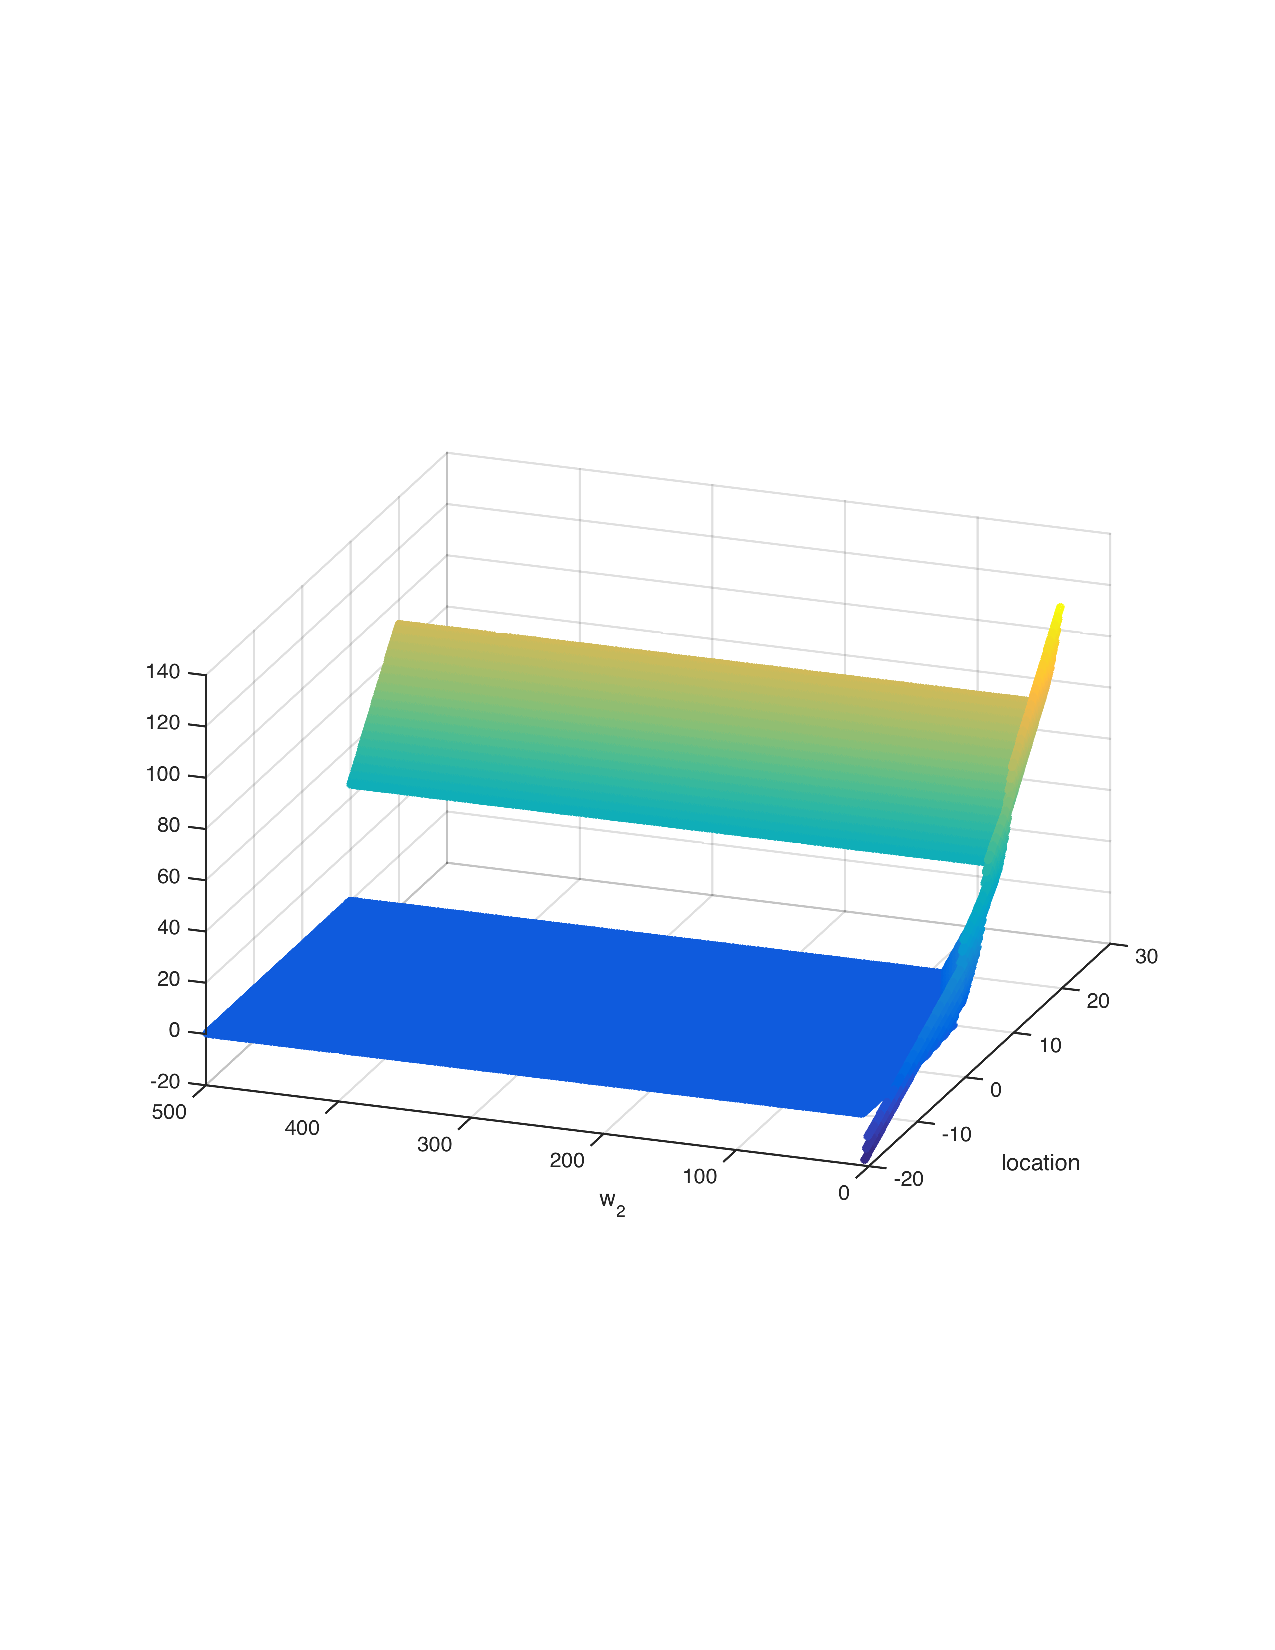
\includegraphics[width=0.8\linewidth, height=0.6\linewidth]{images/robot1d}
    \caption{The optimal value function for the multiobjective navigation domain.}
    \label{fig:vehicle1d}            
\end{figure}
%------------------------------------------------------------------------------

\subsection{Influenza Public Health Policy}
\label{sec:results_influenza}

Influenza viruses continuously challenge both human and avian posts with new variants causing complex epidemics. Compartmental models are widely used within epidemiology to investigate the spread of infection diseases. In this domain we investigate the sensitivity of two different Influenza models to an infection rate parameter. 

\subsubsection{S-I Model}
\label{sec:results_influenza_sd}

A simple epidemiological model is the two compartment S-I, model where {\footnotesize $ s_t $} refers to the number of susceptibles and {\footnotesize $ i_t $} to the number of infected. At each time step the population in each of the three populations is updated according to the following equations:
{\footnotesize
\begin{align*}
    s_{t + 1} &= - s_t \cdot ( \eta + a ) \\
    i_{t+1} &= \eta \cdot s_t 
\end{align*}
}
where {\footnotesize $ \eta \in [0, 1]$} is the rate of infection and {\footnotesize $ a_t \in \left\lbrace 0, \ldots, 1.0\right\rbrace $} is the proportion of susceptibles {\footnotesize $ s_t $} to be vaccinated. The S-I model can be formulated as an parameterized MDP as follows:
\begin{itemize}
    \item {\footnotesize $ \State = \left\langle s, i \right\rangle$ }, where $ s $ and $ i $ are as defined above
    \item {\footnotesize $ \Action \in \left\lbrace 0, 0.25, 0.50, 1.0 \right\rbrace $} is the proportion of $ s $ to vaccinate
    \item The transition function {\footnotesize \Transition} for each state variable in {\footnotesize \State} is given by:    \\
    {\footnotesize 
        \abovedisplayskip=5pt
        \belowdisplayskip=0pt
        \renewcommand{\arraystretch}{1.5}
        \begin{tabular}{ll}
            $ \Transition\left( s' | s, i, a \right) =$ & $ \delta \left[ s' - (- s \cdot (\eta + a)) \right] $ \\
            $ \Transition\left( i' | s, i, a \right) =$ & $ \delta \left[ i' - (\eta \cdot s) \right] $ \\
        \end{tabular}
    }%
    \item {\footnotesize $ \Reward\left(\vec{w}, cost_{\mathtt{inf}}, cost_{\mathtt{vaccine}}, s, i, a \right) = w_1 \cdot \Reward_{\mathtt{inf}} + w_2 \cdot \Reward_{\mathtt{vaccine}}$} where, \\
%    {\footnotesize $ cost_{\mathtt{inf}} $} is the incident cost of infection and {\footnotesize $ cost_{\mathtt{vaccine}} $} is the unit cost of vaccination \\
    {\footnotesize 
        \abovedisplayskip=10pt
        \belowdisplayskip=0pt
        \renewcommand{\arraystretch}{1.5}
        \begin{tabular}{ll}    
            $ \Reward_{\mathtt{inf}}(s', i', a, cost_{\mathtt{inf}}) = $ &  $ $ \\
                \qquad $ \begin{cases}
                (i \geq 0) : & cost_{\mathtt{death}} \cdot i \\
                \text{otherwise} : & 0 \\
                \end{cases} $ & $ $ \\
            $ \Reward_{\mathtt{vaccine}}(s', i', a, cost_{\mathtt{vaccine}}) = $ &  $ $ \\
                \qquad $ \begin{cases}
                (s \geq 0) : & cost_{\mathtt{vaccine}} \cdot s \cdot a \\
                \text{otherwise} : & 0 \\
                \end{cases} $ & $ $ \\
        \end{tabular}
    }    
\end{itemize} 

Figure~\ref{fig:influenza_sd} displays the sensitivity of the optimal {\footnotesize$ \Horizon = 4 $} value function for the S-I model to infection rate parameter {\footnotesize $ \eta \in \left\lbrace 0, 0.02 \right\rbrace$}. The parameters of the models were set to {\footnotesize $cost_{\mathtt{inf}} = 95.0$} and {\footnotesize$cost_{\mathtt{vaccine}} = 33.0$}. From the Figure it is clear that as the number of susceptibles {\footnotesize $ s $} increases, an increase in the infection rate parameter {\footnotesize $ \eta $}, leads to a deleterious outcome for the population.
%------------------------------------------------------------------------------
% Figure
\begin{figure}[h!]
    \centering
    \begin{subfigure}[b]{0.4\textwidth}    
        %        \centering
        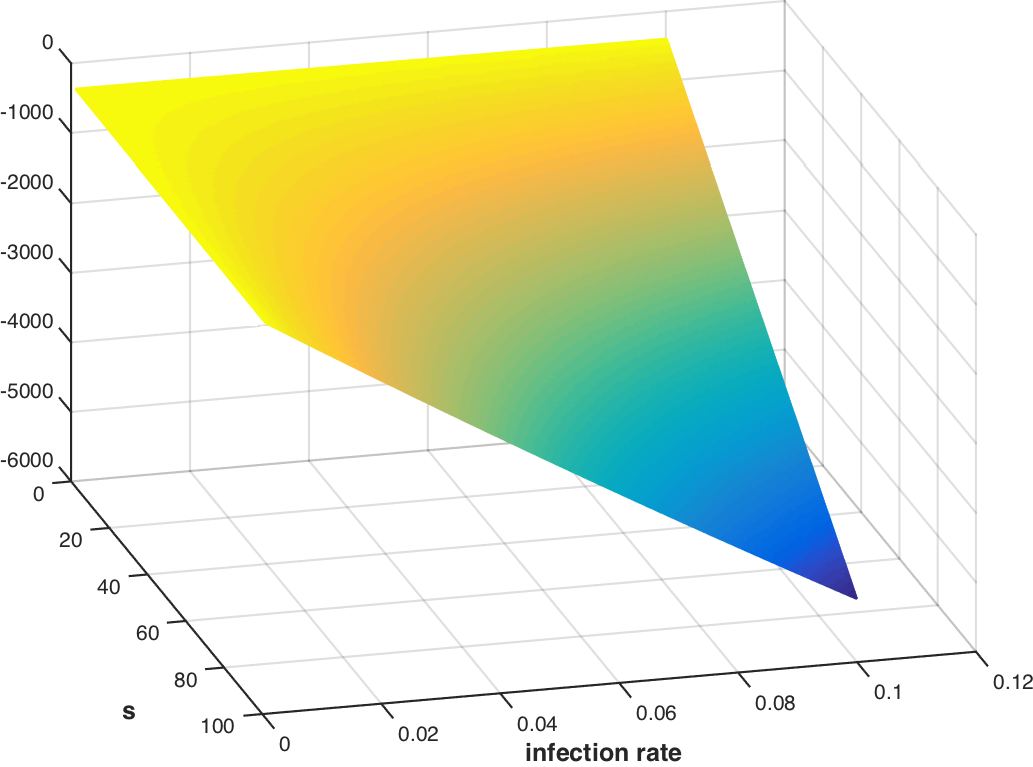
\includegraphics[width=0.8\linewidth, height=0.6\linewidth]{images/sd_infection_s}
        \caption{Optimal Influenza Epidemiology value under the S-D specification.}
        \label{fig:influenza_sd_value_function}
        \vspace{1em}
    \end{subfigure}
    
    \begin{subfigure}[b]{0.4\textwidth}    
        %        \centering
    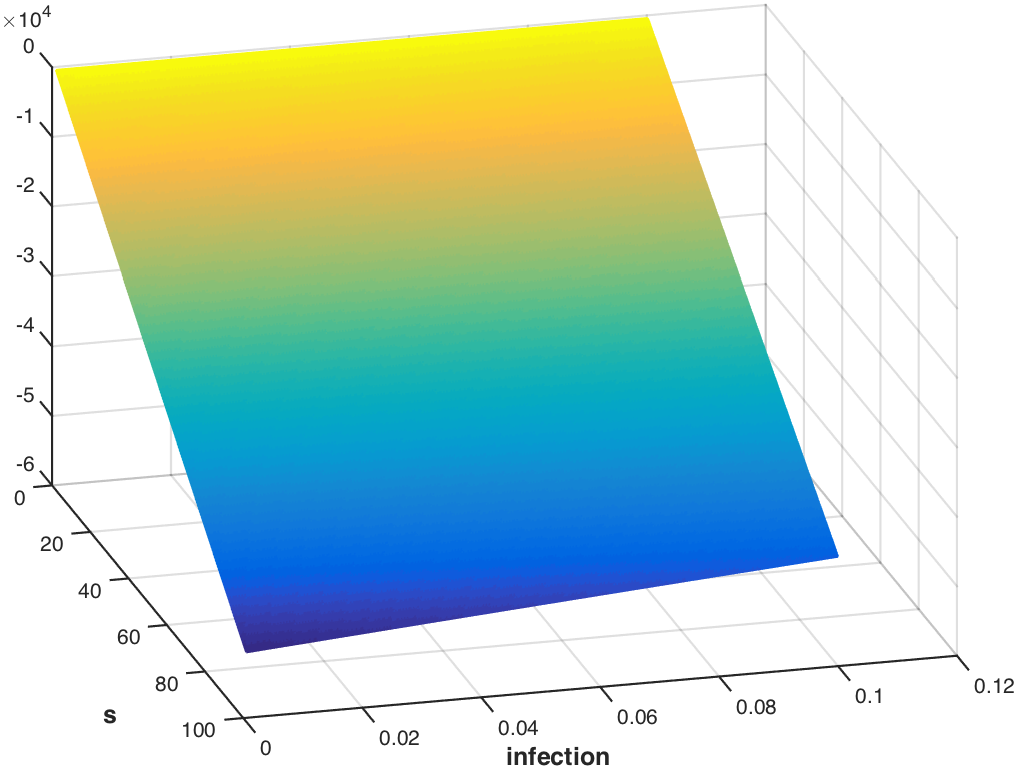
\includegraphics[width=0.8\linewidth, height=0.6\linewidth]{images/sd_infection_sensitivity}
    \caption{Sensitivity.}
    \label{fig:influenza_sd_sensitivity}
    \end{subfigure}  
    \caption{The optimal value function for the S-D model.}
    \label{fig:influenza_sd}    
\end{figure}
%------------------------------------------------------------------------------

\subsubsection{S-I-R-S Model}
\label{sec:results_influenza_sirs}

A more complex epidemiological model is the three compartment S-I-R-S, model where {\footnotesize $ s_t $} refers to the number of susceptibles, {\footnotesize $ i_t $} to number of infected and {\footnotesize $ r_t $} to the recovered. At each time step the population in each of the three populations is updated according to the following equations:
{\footnotesize
\begin{align*}
    s_{t + 1} &= -\eta \cdot s_t \cdot i_t + \lambda \cdot r_t - a_t \cdot s_t \\
    i_{t + 1} &= \eta \cdot s_t \cdot i_t - \beta \cdot i_t \\
    r_{t+1} &= \beta \cdot i_t - \lambda \cdot r_t 
    %    d_{t+1} &= e \cdot i_t 
\end{align*}
}
where {\footnotesize $ \eta \in [0, 1]$} is the rate of infection, {\footnotesize $ \beta \in [0, 1]$} is the rate of recovery and {\footnotesize $ \lambda \in [0, 1]$} is the rate of susceptibility, and {\footnotesize $ a_t \in \left\lbrace 0, \ldots, 1.0\right\rbrace $} is the proportion of susceptibles {\footnotesize $ s_t $} to be vaccinated. The S-I-R-S model can be formulated as an parameterized MDP as follows:
\begin{itemize}
    \item {\footnotesize $ \State = \left\langle s, i, r \right\rangle$ }, where $ s $, $ i $, and $ r $ are as defined above
    \item {\footnotesize $ \Action \in \left\lbrace 0, 0.25, 0.50, 1.0 \right\rbrace $} is the proportion of $ s $ to vaccinate
    \item The transition function {\footnotesize \Transition} for each state variable in {\footnotesize \State} is given by:    \\
    {\footnotesize 
        \abovedisplayskip=5pt
        \belowdisplayskip=0pt
        \renewcommand{\arraystretch}{1.5}
        \begin{tabular}{ll}
            $ \Transition\left( s' | s, i, r, a \right) =$ & $ \delta \left[ s' - (- \eta \cdot s \cdot i + \lambda \cdot r -a \cdot s) \right] $ \\
            $ \Transition\left( i' | s, i, r, a \right) =$ & $ \delta \left[ i' - (\eta \cdot s \cdot i - \beta \cdot i) \right] $ \\
            $ \Transition\left( r' | s, i, r, a \right) =$ & $ \delta \left[ r' - (\beta \cdot i - \lambda \cdot r) \right] $ \\            
        \end{tabular}
    }%
    \item {\footnotesize $ \Reward\left(\vec{w}, cost_{\mathtt{inf}}, cost_{\mathtt{vaccine}}, s, i, r, a \right) = w_1 \cdot \Reward_{\mathtt{inf}} + w_2 \cdot \Reward_{\mathtt{vaccine}}$} where, \\
%    {\footnotesize $ cost_{\mathtt{inf}} $} is the incident cost of infection and {\footnotesize $ cost_{\mathtt{vaccine}} $} is the unit cost of vaccination \\
    {\footnotesize 
        \abovedisplayskip=10pt
        \belowdisplayskip=0pt
        \renewcommand{\arraystretch}{1.5}
        \begin{tabular}{ll}    
            $ \Reward_{\mathtt{inf}}(s', i', r', a, cost_{\mathtt{death}}) = $ &  $ $ \\
            \qquad $ \begin{cases}
            (i \geq 0) : & cost_{\mathtt{death}} \cdot i \\
            \text{otherwise} : & 0 \\
            \end{cases} $ & $ $ \\
            $ \Reward_{\mathtt{vaccine}}(s', i', a, cost_{\mathtt{vaccine}}) = $ &  $ $ \\
            \qquad $ \begin{cases}
            (s \geq 0) : & cost_{\mathtt{vaccine}} \cdot s \cdot a \\
            \text{otherwise} : & 0 \\
            \end{cases} $ & $ $ \\
        \end{tabular}
    }    
%    \item {\footnotesize $ \Reward\left(\vec{w}, cost_{\mathtt{inf}}, s, i, r, a \right) = w_1 \cdot -cost_{\mathtt{inf}} \cdot i + w_2 \cdot -cost_{\mathtt{vaccine}} \cdot a $}, where {\footnotesize $ cost_{\mathtt{inf}} $} is the incident cost of infection and {\footnotesize $ cost_{\mathtt{vaccine}} $} is the unit cost of vaccination \\
\end{itemize} 

Figure~\ref{fig:influenza_sirs} displays the sensitivity of the optimal {\footnotesize$ \Horizon = 4 $} value function for the S-I-R-S model to infection rate parameter {\footnotesize $ \eta \in \left\lbrace 0, 0.02 \right\rbrace$}. The parameters of the models were set to {\footnotesize$ \beta = 0.27, \lambda = 0.23, cost_{\mathtt{inf}} = 95.0$} and {\footnotesize$cost_{\mathtt{vaccine}} = 33.0$}. From the Figure it is clear that the deleterious affect of an increasing {\footnotesize $ \eta $} is counteracted by the amount of individuals becoming susceptible due to the rate of susceptibility {\footnotesize $ \lambda $}.
%------------------------------------------------------------------------------
% Figure
\begin{figure}[t!]
    \centering
    \begin{subfigure}[b]{0.4\textwidth}    
        %        \centering
        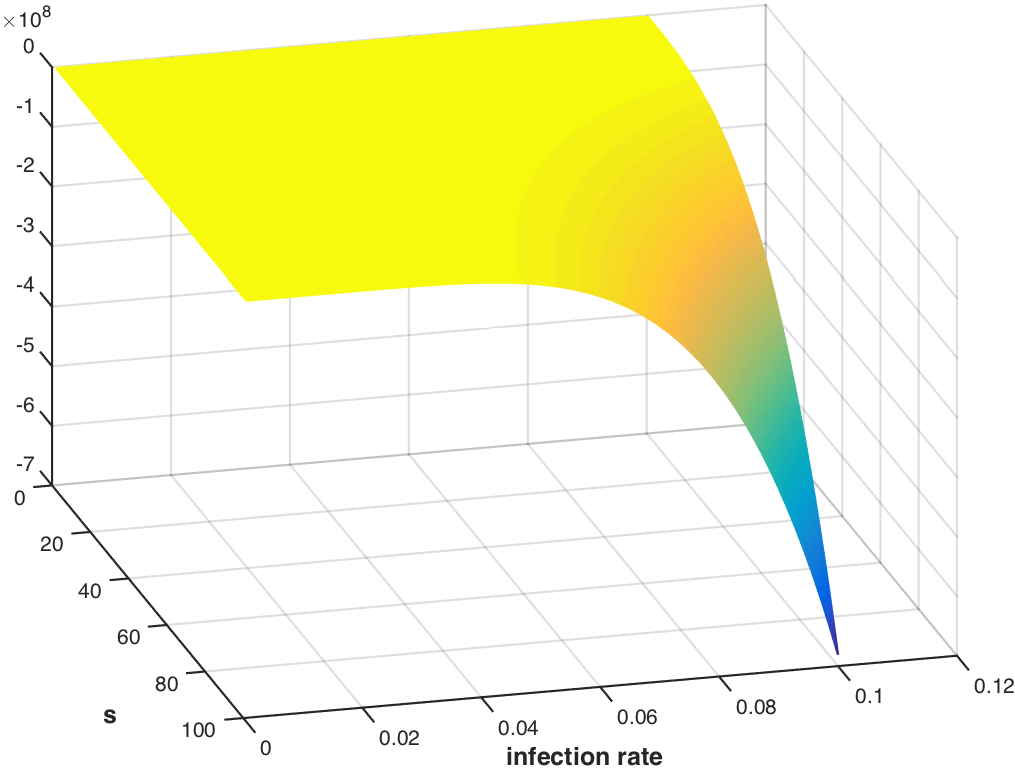
\includegraphics[width=0.8\linewidth, height=0.6\linewidth]{images/sir_infection_s}
        \caption{Optimal Influenza Epidemiology value under the S-I-R-S specification.}
        \label{fig:influenza_sirs_value_function}
        \vspace{1em}
    \end{subfigure}
    
    \begin{subfigure}[b]{0.4\textwidth}    
        %        \centering
        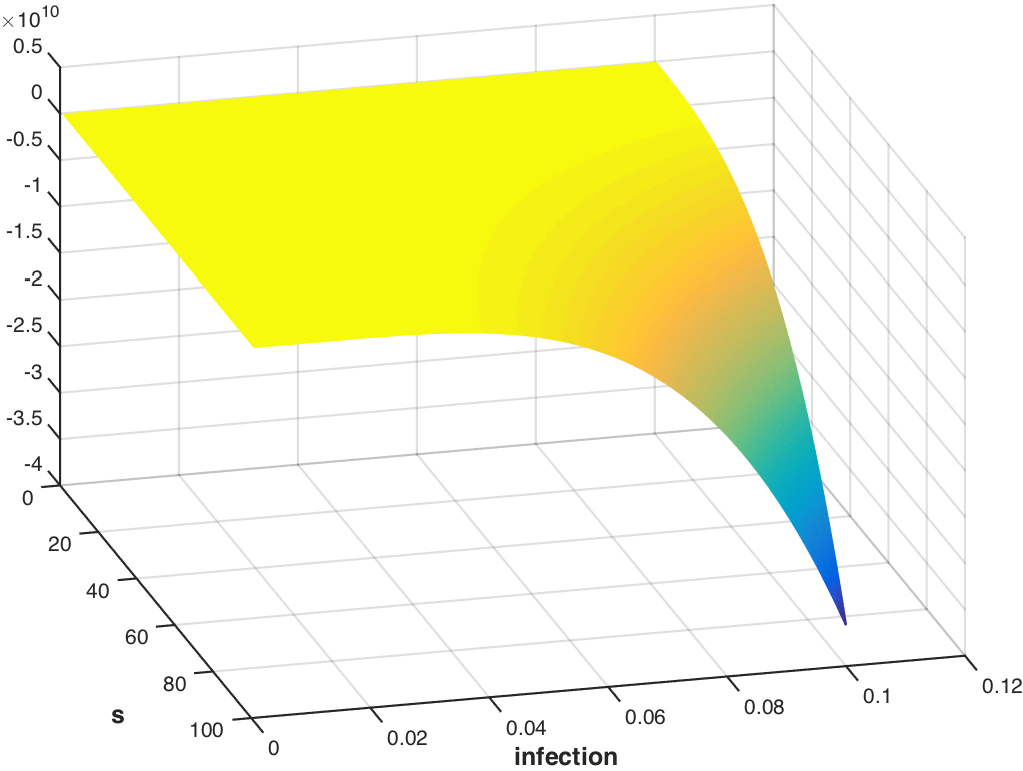
\includegraphics[width=0.8\linewidth, height=0.6\linewidth]{images/sir_infection_sensitivity}
        \caption{Sensitivity.}
        \label{fig:influenza_sirs_sensitivity}
    \end{subfigure}  
    \caption{The optimal value function for the S-I-R-S model.}
    \label{fig:influenza_sirs}      
\end{figure}
%------------------------------------------------------------------------------

\subsection{Optimal Execution}
\label{sec:results_oe}

Institutional investors often need to acquire or liquidate a number of shares within a given period of time. Indirect transaction costs are an important consideration for institutional investors who often want to transact a number of shares that exceeds the available liquidity i.e. there may not be counterparty or counterparties that wish to take the other side of the trade at the same volume. There is a clear trade-off between the market impact of transacting immediately and the volatility of slow execution. 

In this domain we use a price impact model inspired by Bertsimas and Lo~\parencite{Bertsimas_JFM_1998} to investigate the optimisation of parameters within two static policies: (1) constant liquidation; and (2) fractional liquidation. The common components of the optimal execution domain for each type of static policy can be defined as:
\begin{itemize}
    \item {\footnotesize $ \State = \left\langle price, inv \right\rangle$}, where $ price $ is the price of the asset and $ inv $ is the inventory remaining
    \item  {\footnotesize $ \Transition\left( price' | price, inv, a \right) = \delta \left[ price' - (price + \kappa + \sigma \cdot \epsilon) \right] $}
\end{itemize}

\subsubsection{Constant Liquidation Policy}
\label{sec:results_oe_constant}

With a constant liquidation policy the investor chooses to sell a constant number of assets at each time period. This specific scenario is defined by the following:
\begin{itemize}
    \item {\footnotesize 
         \begin{tabular}{ll}
            $ \Transition\left( inv' | price, inv, a \right) = $ & $ $ \\
            $ \qquad \delta \left[ inv' - \begin{cases}
            inv \geq a : & inv - a \\
            \text{otherwise} : & inv \\
            \end{cases} \right] $ & $ $\\
        \end{tabular}
    }%
    \item {\footnotesize $ \Reward\left(price, price_0, inv, a \right) =
        \begin{cases}
            (inv \geq a) : & a \cdot price - a \cdot price_0 \\
            \text{otherwise} : & 0 \\
        \end{cases} $}
    \item {\footnotesize $ \Action \in \left\lbrace 0, \ldots, inv \right\rbrace $} is the number of the remaining inventory to sell    
\end{itemize}

\subsubsection{Fractional Liquidation Policy}
\label{sec:results_or_fractional}

With a fractional liquidation policy the investor chooses to sell a constant proportion of assets at each time period. This specific scenario is defined by the following:
\begin{itemize}
    \item {\footnotesize $\Transition\left( inv' | price, inv, n \right) = \delta \left[ inv' - (inv - inv \cdot a) \right] $}
    \item {\footnotesize $ \Reward\left(price, price_0, inv, a \right) =
        \begin{cases}
        (inv \geq a) : & a \cdot inv \cdot price - inv \cdot price_0 \\
        \text{otherwise} : & 0 \\
        \end{cases} $} 
    \item {\footnotesize $ \Action \in \left\lbrace 0, 0.25, 0.50, 1.0 \right\rbrace $} is the proportion of the remaining inventory to sell    
\end{itemize}

The investor aims to minimise implementation shortfall, which is defined as the difference between the theoretical benchmark price and the actual price received is the implementation shortfall~\parencite{Perold_JPM_1988}.

Figure~\ref{fig:opt_execution} displays the sensitivity of the optimal {\footnotesize$ \Horizon = 5 $} value function for the optimal execution model under both static policies. The parameters of the models were set to {\footnotesize$ \kappa = 0.0.0165, price_0 = 10.0, price = 20.0$} and {\footnotesize$inv = 200.0$}. 
%------------------------------------------------------------------------------
% Figure
\begin{figure}[t!]
    \centering
    \begin{subfigure}[b]{0.4\textwidth}    
%        \centering
        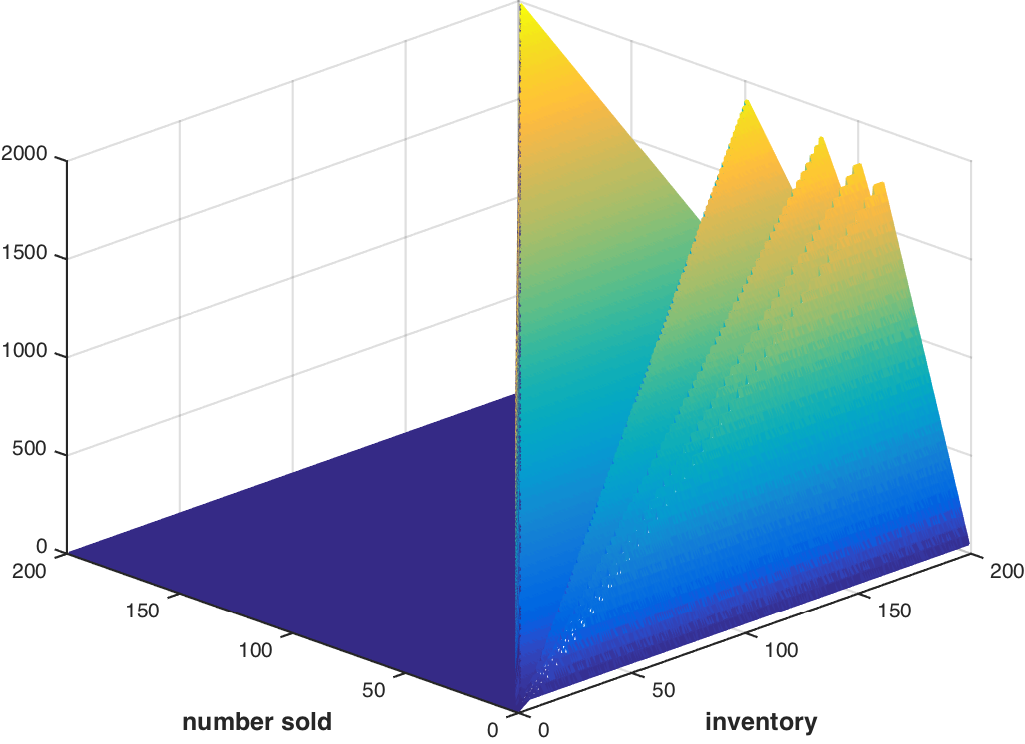
\includegraphics[width=\linewidth, height=0.6\linewidth]{images/opt_execution_budget}
        \caption{Constant liquidation.}
        \label{fig:opt_execution_w1}
        \vspace{1em}
    \end{subfigure}
    
    \begin{subfigure}[b]{0.4\textwidth}    
%        \centering
        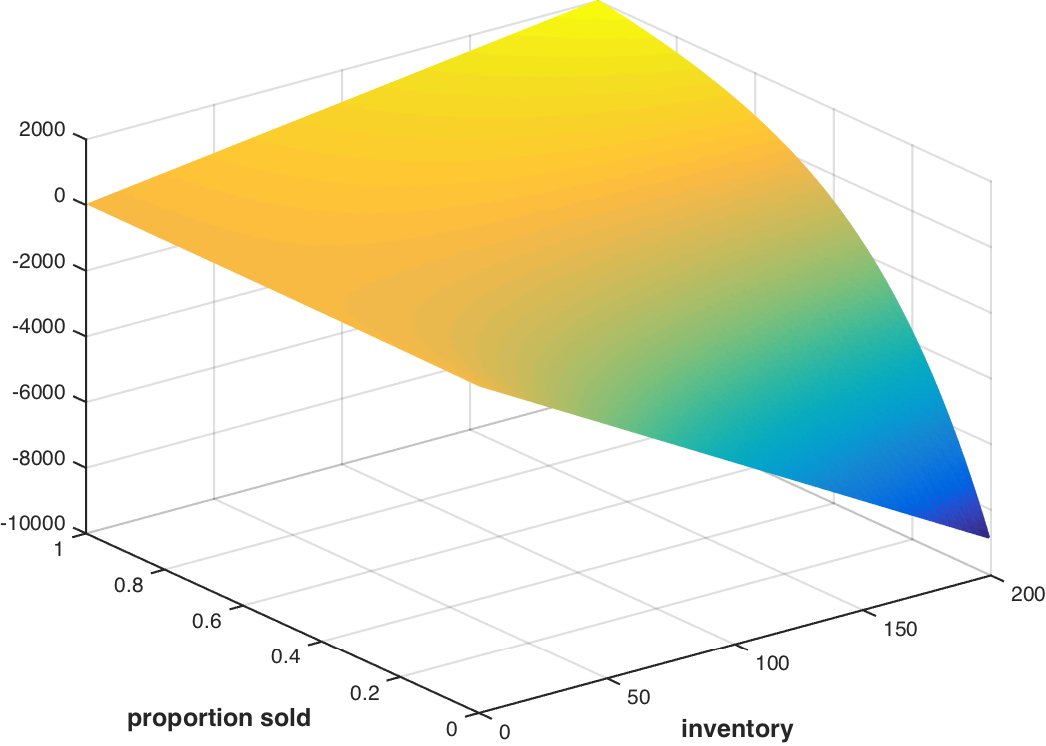
\includegraphics[width=\linewidth, height=0.6\linewidth]{images/opt_execution_fraction}
        \caption{Fractional liquidation.}
        \label{fig:opt_execution_w2}
    \end{subfigure}  
    \caption{The optimal execution value function under different policies.}
    \label{fig:opt_execution}
\end{figure}
%------------------------------------------------------------------------------